%%%%%%%%%%%%%%%%%%%%%%%%%%%%%%%%%%%%%%%%%%%%%%%%%%%%%%%%%%%%%%%%%%%%%%%%%%%%
%% Author template for Operations Reseacrh (opre) for articles with no e-companion (EC)
%% Mirko Janc, Ph.D., INFORMS, mirko.janc@informs.org
%% ver. 0.95, December 2010
%%%%%%%%%%%%%%%%%%%%%%%%%%%%%%%%%%%%%%%%%%%%%%%%%%%%%%%%%%%%%%%%%%%%%%%%%%%%
%\documentclass[opre,blindrev]{informs3}
\documentclass[opre,nonblindrev]{informs3} % current default for manuscript submission

%%%%%%%%%%%%%%%%%%%%%%%%%%%%%%%%%%%%%%%%%%%%%%%%%%
%% added packages and commands
% to include comments in the generated pdf comment the \commfalse and uncomment \commtrue
\newif\ifcomm
\commtrue
%\commfalse

\usepackage{mathtools}
\usepackage{comment}
\usepackage{float}
\usepackage{hyperref}
\usepackage{epsfig}
\usepackage{xspace}
\usepackage{balance}
\usepackage{subcaption}
%\usepackage{caption}
\usepackage[margin=10pt,labelfont=bf,font={footnotesize}]{caption}
\usepackage{bbm}
\usepackage{url}
%\usepackage{cases}
%\usepackage{color}
%\usepackage[ruled,vlined,linesnumbered]{algorithm2e}
\usepackage{algorithm}
\usepackage[noend]{algpseudocode}
\usepackage{times}
\usepackage{amsthm}
\usepackage{amsmath, graphicx, latexsym, amssymb,  amsfonts}
\newcommand{\T}[1]{\smallskip\noindent\textbf{#1}} %paragraph title

\newtheorem{lemma}{Lemma}
\newtheorem{corollary}{Corollary}
\newtheorem{theorem}{Theorem}
\newtheorem{proposition}{Proposition}

\renewcommand{\proof}{\noindent{\bf Proof.\ }}

%%%%%%%%%%%%%%%%%%%%%%%%%%%%%%%%%%%%%%%%%%%%%%%%%%%%%%
\makeatletter
\newtheorem*{rep@theorem}{\rep@title}
\newcommand{\newreptheorem}[2]{%
\newenvironment{rep#1}[1]{%
 \def\rep@title{#2 \ref{##1}}%
 \begin{rep@theorem}}%
 {\end{rep@theorem}}}
\makeatother
\newreptheorem{theorem}{Theorem}
\newreptheorem{proposition}{Proposition}
\newreptheorem{lemma}{Lemma}
\newtheorem{remark}{Remark}
%%%%%%%%%%%%%%%%%%%%%%%%%%%%%%%%%%%%%%%%%%%%%%%%%%%%%%
%%%%%%%%%%%%%%%%%%%%%%%%%%%%%%%%%%%%%%%%%%%%%%%%%%%%%%
\newcommand{\twopartdefifelse}[3]
{
	\left\{
		\begin{array}{ll}
			#1, & \quad\mbox{if } #2, \\
			#3, & \quad \mbox{otherwise.}
		\end{array}
	\right.
}
\newcommand{\twopartdef}[4]
{
	\left\{
		\begin{array}{ll}
			#1, & \quad\mbox{if } #2, \\
			#3, & \quad\mbox{if } #4
		\end{array}
	\right.
}

\newcommand{\threepartdef}[6]
{
	\left\{
		\begin{array}{lll}
			#1, & \quad\mbox{if } \quad #2, \\
			#3, & \quad\mbox{if } \quad #4, \\
			#5, & \quad\mbox{if } \quad  #6.
		\end{array}
	\right.
}
%========================
%  Defining comments
%========================

\ifcomm
    \newcounter{commentNumberI}
    \setcounter{commentNumberI}{0}
    
    % (1) comments in color or bold
     \newcommand{\Eyal}[1]{\addtocounter{commentNumberI}{1}{{({\color{blue} {(\arabic{commentNumberI}.)} Eyal: #1})}}} %just color
       \newcommand{\Gal}[1]{\addtocounter{commentNumberI}{1}{{({\color{red} {(\arabic{commentNumberI}.)} Gal: #1})}}} %just color
    \newcommand{\A}[1]{\textbf{[#1]}}       %Comments -> in bold

    % (2) comments in footnote
    \newcommand{\F}[1]{\footnote {\color{red} [#1]}}

\else
    \newcommand{\A}[1]{}
    \newcommand{\Eyal}[1]{}
    \newcommand{\Gal}[1]{}
\fi
\newcommand{\Ey}[1]{\Eyal{#1}}
\newcommand{\GM}[1]{\Gal{#1}}

%%%%%%%%%%%%%%%%%%%%%%%%%%%%%%%%%%%%%%%%%%%%%%%%%

\DoubleSpacedXI % Made default 4/4/2014 at request
%%\OneAndAHalfSpacedXI % current default line spacing
%%\OneAndAHalfSpacedXII
%%\DoubleSpacedXII

% If hyperref is used, dvi-to-ps driver of choice must be declared as
%   an additional option to the \documentclass. For example
%\documentclass[dvips,opre]{informs3}      % if dvips is used
%\documentclass[dvipsone,opre]{informs3}   % if dvipsone is used, etc.

%%% OPRE uses endnotes. If you do not use them, put a percent sign before
%%% the \theendnotes command. This template does show how to use them.
\usepackage{endnotes}
\let\footnote=\endnote
\let\enotesize=\normalsize
\def\notesname{Endnotes}%
\def\makeenmark{$^{\theenmark}$}
\def\enoteformat{\rightskip0pt\leftskip0pt\parindent=1.75em
  \leavevmode\llap{\theenmark.\enskip}}

% Private macros here (check that there is no clash with the style)

% Natbib setup for author-year style
\usepackage{natbib}
 \bibpunct[, ]{(}{)}{,}{a}{}{,}%
 \def\bibfont{\small}%
 \def\bibsep{\smallskipamount}%
 \def\bibhang{24pt}%
 \def\newblock{\ }%
 \def\BIBand{and}%

%% Setup of theorem styles. Outcomment only one.
%% Preferred default is the first option.  
%\TheoremsNumberedThrough
%\TheoremsNumberedByChapter  % (Theorem 1.1, Lema 1.1, Theorem 1.2)
\ECRepeatTheorems

%% Setup of the equation numbering system. Outcomment only one.
%% Preferred default is the first option.
\EquationsNumberedThrough    % Default: (1), (2), ...
%\EquationsNumberedBySection % (1.1), (1.2), ...

% In the reviewing and copyediting stage enter the manuscript number.
%\MANUSCRIPTNO{} % When the article is logged in and DOI assigned to it,
                 %   this manuscript number is no longer necessary


%%%%%%%%%%%%%%%%
\begin{document}
%%%%%%%%%%%%%%%%

% Outcomment only when entries are known. Otherwise leave as is and
%   default values will be used.
%\setcounter{page}{1}
%\VOLUME{00}%
%\NO{0}%
%\MONTH{Xxxxx}% (month or a similar seasonal id)
%\YEAR{0000}% e.g., 2005
%\FIRSTPAGE{000}%
%\LASTPAGE{000}%
%\SHORTYEAR{00}% shortened year (two-digit)
%\ISSUE{0000} %
%\LONGFIRSTPAGE{0001} %
%\DOI{10.1287/xxxx.0000.0000}%

% Author's names for the running heads
% Sample depending on the number of authors;
% \RUNAUTHOR{Jones}
% \RUNAUTHOR{Jones and Wilson}
% \RUNAUTHOR{Jones, Miller, and Wilson}
% \RUNAUTHOR{Jones et al.} % for four or more authors
% Enter authors following the given pattern:
\RUNAUTHOR{}

% Title or shortened title suitable for running heads. Sample:
% \RUNTITLE{Bundling Information Goods of Decreasing Value}
% Enter the (shortened) title:
%\RUNTITLE{Server Slowdown Detection}
\RUNTITLE{MAB Reaction to Shock}

% Full title. Sample:
% \TITLE{Bundling Information Goods of Decreasing Value}
% Enter the full title:
% \TITLE{Service Slowdown Detection}
\TITLE{ MAB Reaction to Shock}

% Block of authors and their affiliations starts here:
% NOTE: Authors with same affiliation, if the order of authors allows,
%   should be entered in ONE field, separated by a comma.
%   \EMAIL field can be repeated if more than one author
\ARTICLEAUTHORS{%
\AUTHOR{}
\AFF{\EMAIL{}
\AUTHOR{}
\AFF{ \EMAIL{}} %, \URL{}}
}
% Enter all authors
} % end of the block

%%%%%%%%%%%%%%%%%%%%%%%%%%%%%%%%%%%%%%%%%%%%%%%%%%%%%%%%%%%%%%%%%%%%%%%%%%%%%%%%%%%%%%%%%%%%%%%%%%%%%%%%%%%%%%
\ABSTRACT{ 

}

%%%%%%%%%%%%%%%%%%%%%%%%%%%%%%%%%%%%%%%%%%%%%%%%%%%%%%%%%%%%%%%%%%%%%%%%%%%%%%%%%%%%%%%%%%%%%%%%%%%%%%%%%%%%%%

% Sample
%\KEYWORDS{deterministic inventory theory; infinite linear programming duality;
%  existence of optimal policies; semi-Markov decision process; cyclic schedule}

% Fill in data. If unknown, outcomment the field
%\KEYWORDS{butter, margarine, silliness} 
%\HISTORY{This paper was
%first submitted on April 12, 1922 and has been with the authors for
%83 years for 65 revisions.}

\maketitle
%%%%%%%%%%%%%%%%%%%%%%%%%%%%%%%%%%%%%%%%%%%%%%%%%%%%%%%%%%%%%%%%%%%%%%

% Samples of sectioning (and labeling) in OPRE
% NOTE: (1) \section and \subsection do NOT end with a period
%       (2) \subsubsection and lower need end punctuation
%       (3) capitalization is as shown (title style).
%
%\section{Introduction.}\label{intro} %%1.
%\subsection{Duality and the Classical EOQ Problem.}\label{class-EOQ} %% 1.1.
%\subsection{Outline.}\label{outline1} %% 1.2.
%\subsubsection{Cyclic Schedules for the General Deterministic SMDP.}
%  \label{cyclic-schedules} %% 1.2.1
%\section{Problem Description.}\label{problemdescription} %% 2.

% Text of your paper here
%\tableofcontents

%%%%%%%%%%%%%%%%%%%%%%%%%%%%%%%%%%%%%%%%%%%%%%%%%%%%%%%%%%
\section{Motivation and background}
The Upper Confidence Bound (UCB) algorithm is a popular approach used in the context of multi-armed bandit problems. In such problems, an agent must decide which arm (or action) to pull from a set of arms, each with an associated unknown reward distribution. The objective is to maximize the cumulative reward over a series of trials.
Multi armed bandits algorithms can be used for network routing, recommendation systems, online advertising, clinical trials etc.
The UCB algorithm addresses the exploration-exploitation dilemma by balancing between exploiting arms with high observed rewards and exploring arms with uncertain rewards. The main idea behind UCB is to use confidence bounds on the estimated rewards to determine which arm to pull at each step.
The simple UCB algorithm assumes that the reward distribution of the arms is stationary which is not true for most practical applications. For example, In network communication, routing packets through different paths can be modeled as a multi-armed bandit problem. The quality or congestion level of network paths may change abruptly due to network failures or traffic fluctuations.
In this project we will study the effect of abrupt changes in the arms rewards distribution on the UCB algorithm’s decisions.


\section{Problem Definition}
First we define the notation and setting of the simple multi armed bandit problem and introduce a few algorithms. We will follow the explanation from \cite{reference1}. A stationary stochastic bandit is a set of distributions $\nu=(P_a:a\in\mathcal{A})$ where $\mathcal{A}$ is the set of available options. The learner and the environment interact sequentially over $n$ rounds. In each round $t \in \{1, \ldots, T\}$, the learner chooses an action $a_t \in \mathcal{A}$, which is fed to the environment. The environment then samples a reward $X_t(a_t) \in \mathbb{R}$ from distribution $P_{a_t}$ and reveals $X_t(a_t)$ to the learner. The objective of the learner is to maximize its cumulative expected reward. The UCB algorithm attempts to do that.

We denote $\mu_i(t)$ to be the mean of the distribution of the $i$'th arm at round t. In the stationary case we write it as $\mu_i$ as the mean remains constant.
Denote
\[
\begin{aligned}
    N_i(t) = \sum\limits_{s=1}^{t}\mathbbm{1}_{(a_s=i)}, & \quad \hat{\mu}_{t,j} = \frac{\sum\limits_{s=1}^{t}X_s(j)\mathbbm{1}_{(a_s=i)}}{N_j(t)}, & K = |\mathcal{A}|
\end{aligned}
\]
$N_i(t)$ the number of times arm i has been played in the first $t$ rounds and $\hat{\mu}_{t,j}$ is the empirical average reward from arm j up to round t.

% Consider the Multi-Armed Bandit problem with $K$ arms, time horizon $T$, and denote by $X_t(i)$ the random reward that would be received if arm $i$ were played in round $t$. At each round, the player picks an arm $I_t\in \{1,\ldots,K\}$ according to a policy/algorithm based on the sequence of past plays and rewards and obtains a reward $X_{t}(I_t)$. We assume the random variables $X_t(i)\sim Bern({\mu_i})$ are independent between arms and rounds. Denote $N_i(t) = \sum\limits_{s=1}^{t}\mathbbm{1}_{(I_s=i)}$ the number of times arm i has been played in the first $t$ rounds.
\begin{algorithm}
\caption{UCB1}
\textbf{Input:} parameter $\alpha$ 
\begin{enumerate}
    \item for $t = 1$ to $K$: play each arm once.
    \item for $t = K+1$ to $T$: play arm j that maximizes the UCB index defined below. $$UCB_{t-1,j} = \hat{\mu}_{t-1,j} + \sqrt{\frac{\alpha\ln{(t-1)}}{N_i(t-1)}}$$
\end{enumerate}
To break ties play the arm with the minimal index.
\end{algorithm}

Another version of UCB1 that requires knowledge of $T$ has a different UCB index, with the only change being that $lnt$ was replaced with $T$. We call this version \textbf{Finite horizon UCB}.

Another algorithm called \textbf{Deterministic $\epsilon$-greedy}, accepts a parameter $\epsilon$ and samples one of the sub-optimal arms every $\frac{1}{\epsilon}$ rounds. For simplicity of the proof, we assume that the algorithm has a sample of each arm before the first round. This assumption doesn't make a significant change in the behavior of the algorithm but allows for more elegant results and analysis.
\begin{algorithm}
\caption{Deterministic $\epsilon$-greedy}
\textbf{Input:} parameter $\epsilon$ such that $\frac{1}{\epsilon}\in \mathbb{N}$, a sample from each arm.
\begin{enumerate}
    \item for $t = K+1$ to $T$:
    \begin{enumerate}
        \item If $t = \frac{k}{\epsilon}$ for some $k\in \mathbb{N}$, choose the arm with the smallest empirical mean.
        \item Otherwise, choose the arm with the maximum empirical mean.
    \end{enumerate}
\end{enumerate}
To break ties play the arm with the minimal index.
\end{algorithm}

To introduce non-stationarity, we first define a very general definition of a non-stationary bandit. A non-stationary bandit is a collection of $T$ distributions for each of the arms (actions) $\nu=(\{P_a(t)\}_{t=1}^{T}:a\in\mathcal{A})$.
A \textbf{change point} is any round where the reward distribution of at least one arm changed. In other words, for $t \in \{2, \ldots, T\}$, round $t$ is a change point if $\exists a\in \mathcal{A}$, $P_a(t-1)\neq P_a(t)$. The first round is not considered to be a change point. To be clear, the change happens before the learner samples the arms at round $t$. In other words, The rewards of round $t$ are based on the new distributions. We mark quantities associated with the optimal arm with *, for example, the optimal arm at round $t$ has mean $\mu^*(t)$.

The regret of a policy $\pi$ on a problem instance $\nu$ is:
    $$R_{\pi}(\nu, T) = \sum\limits_{t=1}^{T}\mu^*(t) - E[\sum\limits_{t=1}^{T}X_t(a_t)]$$
The worst case regret of $\pi$ on a set of problem instances $\mathcal{E}$ is:
$$R_{\pi}(\mathcal{E}, T) = \max_{\nu\in \mathcal{E}} R_{\pi}(\nu, T)$$
When $\mathcal{E}$ and $\pi$ are clear from context, we simply write $R(T)$.
\section{Examples}
Consider the set of non-stationary bandits $\mathcal{E}$ such that $\mathcal{A} = \{1, 2\}$, every instance in $\mathcal{E}$ has at most one change point and $\forall t \in [T], \forall a\in \mathcal{A}$, $P_a(t)$ has support on the interval $[0, 1]$.
\begin{proposition}
    Fix $T>105$ and let $\pi$ be the finite horizon UCB algorithm. Then we have:
    \begin{equation}
        R_\pi(\mathcal{E}, T) \geq 0.7T\Bigg(1-\sqrt{\frac{(0.85T-2)lnT}{2(0.15T-1.5)^2}}\Bigg)
    \end{equation}
    Notice that $\lim_{{T \to \infty}}\frac{R(\nu, T)}{T} = 0.7$.
    \label{prop:UCB_weak_lower_bound}
\end{proposition}

\begin{proof}
To prove that statement we find an instance $\nu \in \mathcal{E}$ such that the regret is at least $0.7T$. We consider the instance where the arms distributions are deterministic for each $t$, so we can describe the distributions of the arms at every round using a pair of values, $(\mu_1(t), \mu_2(t))$ such that $P(X_i(t)=\mu_i(t)) = 1$. We choose the change point to be
\[ c = 
\begin{cases}
    \lfloor0.3T\rfloor & \text{if $\lfloor0.3T\rfloor$ is odd,} \\
    \lfloor0.3T\rfloor-1 & \text{otherwise}.
\end{cases}
\]
The means of the arms in $\nu$ are: $(0, 0)$ for $t<c$ and $(\Delta,1)$ otherwise, where $\Delta := \sqrt{\frac{(0.85T-2)lnT}{2(0.15T-1.5)^2}}$. \\
Notice that $0 < \Delta < 1$ for $T > 105$ (Will be proved at the end).
First we prove by induction that $\forall t\leq c$, if $t$ is odd then $a_t = 1$ and if $t$ is even then $a_t = 2$.

We use strong induction. For the base case, we know that the claim applies for the first two rounds because of the initialization part of the algorithm. Assume the claim holds up to round $t<c$ (including round $t$). Notice that for every $t<c$, $\hat{\mu}_{t, 1} = \hat{\mu}_{t, 2} = 0$.\\
If $t$ is even, then $a_t = 2$. Also $N_2(t) = N_1(t) = \frac{t}{2}$, and therefore $UCB_{t, 1} = UCB_{t, 2}$. Because of the tie breaking policy, we can tell that $a_{t+1} = 1$.\\
If $t$ is odd, then $a_t = 1$. Also $N_1(t) = N_2(t) + 1 = \frac{t-1}{2} + 1$, and therefore $UCB_{t, 1} < UCB_{t, 2}$. Therefore $a_{t+1} = 2$ and we proved the claim.

The regret up to round $c$ is 0. Next we prove by induction that $c \leq \forall t \leq T$, $a_t = 1$. Assuming this is true, $R(\nu, T) \geq 0.7T(1-\Delta)$.

Because of the first claim, in round $c$, UCB picks arm 1 and gets a reward of $\Delta$.\\
Assume that the induction hypothesis is true up to round $t-1$. Denote $\gamma := \frac{c-1}{2}$ and for every $c \leq s \leq t$, $x := s - c$. Notice that $\gamma = N_1(c-1) = N_2(c-1)$ and $x$ is the number of rounds since the change point until round $s$.
Then by the induction hypothesis $f(x) := UCB_{s-1, 1} = \frac{\Delta x}{\gamma + x} + \sqrt{\frac{2lnT}{\gamma + x}}$ and $UCB_{s-1, 2} = \sqrt{\frac{2lnT}{\gamma}}$ for every $c \leq s \leq t \iff 0 \leq x \leq t-c$. \\
We need to show that $f(t-c) = UCB_{t-1, 1} > \sqrt{\frac{2lnT}{\gamma}} = f(0) = UCB_{t-1, 2}$. 
Taking the derivative of $f(x)$ we get $$f'(x) = \frac{\Delta\gamma\sqrt{\frac{2lnT}{\gamma+x}}-lnT}{(\gamma+x)^2\sqrt{\frac{2lnT}{\gamma+x}}}$$
\[
f'(x^*) = 0 \implies x^* = \frac{2\Delta^2\gamma^2}{lnT} - \gamma
\]
since $0.3T - 2 < c \leq 0.3T$, $0.15T - 1.5 < \gamma < 0.15T$:
\[
\Delta > \sqrt{\frac{(0.7T-2 + \gamma)lnT}{2\gamma^2}} \implies x^*>0.7T - 2 > T - c
\]
Clearly $x^*$ is a maximum. Therefore $f(x)$ is increasing for $x<x^*$ and therefore $f(t-c) > f(0)$. \\
To see why $\Delta < 1$ for every $T>105$ define $g(x) = \frac{(0.85x-2)lnx}{2(0.15x-1.5)^2}$.
Taking the derivative we get:
$$g'(x) = -\dfrac{10((17x^2+90x)\ln(x)-17x^2+210x-400)}{9(x-10)^3x}$$
for $x>105$ we have $g'(x) < -\dfrac{10(300x-400)}{9(x-10)^3x} < 0$ and therefore $g(x)$ is decreasing for $x > 105$.\\
$g(105) < 1$ and therefore $\Delta<1$ for $x>105$.  
\end{proof}

%%%%%%%%%%%%%%%%%%%%%%%%%%%%%%%%%%%%%%%%%%%%%%%%%%%%%%%%
Consider the set of non-stationary bandits $\mathcal{E}$ such that $\mathcal{A} = \{1, 2\}$, every instance in $\mathcal{E}$ has at most one change point and $\forall t \in [T], \forall a\in \mathcal{A}$, $P_a(t)$ has support on the interval $[0, 1]$. 
\begin{proposition}
    Fix $T\geq12$ and let $\pi$ be the finite horizon UCB algorithm and $\alpha := \sqrt{2lnT}$. Then:
    \begin{equation}
        R_{\pi}(\mathcal{E}, T) \geq (T-\sqrt[3]{2T^2\alpha^2})\bigg(1-\frac{\alpha\sqrt[3]{4}}{\sqrt[3]{T\alpha}}\bigg).
    \end{equation}
    \label{prop:UCB_strong_lower_bound}
\end{proposition}

\begin{proof}
    Fix $T\geq12$.
    To prove the statement we find an instance $\nu \in \mathcal{E}$ for which the regret $R_{\pi}(\nu, T)$ is at least $(T-\sqrt[3]{2T^2\alpha^2})\bigg(1-\frac{\alpha\sqrt[3]{4}}{\sqrt[3]{T\alpha}}\bigg)$.

    Fix $c\in \mathbbm{N}$ such that $2c+1 < T$. Let $\Delta\in(0,1)$. The values of $c$ and $\Delta$ will be determined later in the proof. Assume that the two arms have the following (round dependent) reward distribution:
    $$(\mu_1(t),\mu_2(t))=\twopartdef{(0,0)}{t<2c+1}{(\Delta,1)}{2c+1\leq t\leq T}.$$
    Thus, the rewards are deterministic in each round and there is a single change in the distribution of the rewards at $t=2c+1$.

    First, we argue that up until (and including) time $2c+1$, the policy alternates between the arms such that arm 1 is pulled at odd times and arm 2 is pulled at even times.

    We use strong induction. The base case applies from the definition of the algorithm.
    Assume the claim holds up to round $t<c$ (including round $t$). Notice that for every $t<c$, $\hat{\mu}_{t, 1} = \hat{\mu}_{t, 2} = 0$.\\
    If $t$ is even, then $a_t = 2$. Also $N_2(t) = N_1(t) = \frac{t}{2}$, and therefore $UCB_{t, 1} = UCB_{t, 2}$. Because of the tie breaking policy, we can tell that $a_{t+1} = 1$.\\
    If $t$ is odd, then $a_t = 1$. Also $N_1(t) = N_2(t) + 1 = \frac{t-1}{2} + 1$, and therefore $UCB_{t, 1} < UCB_{t, 2}$. Therefore $a_{t+1} = 2$ and we proved the claim.

    Thus, up to time $2c+1$, each arm was pulled $c$ times. In addition, at time $2c+1$ arm 1 is pulled but now has a reward of $\Delta$ instead of 0. Our goal is to choose the values of $c$ and $\Delta$ such that the policy keeps choosing the sub-optimal arm 1 for the remaining horizon (i.e., for all $2c+2<t\leq T$. In such a case, the regret is:
    $$R_{\pi}(\nu, T)=(T-2c)(1-\Delta).$$
    So, we will derive conditions for $c$ and $\Delta$ under which the policy keeps choosing arm 1, and find $c$ and $\Delta$ that satisfy these conditions for which the regret is at least $(T-\sqrt[3]{2T^2\alpha^2})\bigg(1-\frac{\alpha\sqrt[3]{4}}{\sqrt[3]{T\alpha}}\bigg)$.

\begin{lemma}\label{lem:arm_1_keeps_being_chosen}
    Assume that for all $x\in{0,1,\ldots,T-2c}$ we have that
    $$\frac{\Delta x}{c+x}+\sqrt{\frac{2\ln{T}}{c+x}}\geq \sqrt{\frac{2\ln{T}}{c}}.$$
    Then arm 1 is chosen for all $t\in\{2c+1,\ldots,T\}$.
\end{lemma}
\begin{proof}
    We use strong induction. For the base case, we already know that arm 1 is chosen at time $2c+1$. To understand what happens at $t=2c+2$, we compare the UCB's:
    $$UCB_{2c+1,1}=\frac{\Delta }{c+1}+\sqrt{\frac{2\ln{T}}{c+1}},$$
    and
    $$UCB_{2c+1,2}=\sqrt{\frac{2\ln{T}}{c}}.$$
    By our assumption (with $x=1$), we have that $UCB_{2c+1,1}\geq UCB_{2c+1,2}$ and therefore arm 1 is chosen again at $t=2c+2$. Now, consider a time $2c+2\leq t \leq T-1$ and assume that arm 1 is chosen up until and including time $t$. Then, we must have 
    $$UCB_{t,1}=\frac{\Delta }{c+(t-2c)}+\sqrt{\frac{2\ln{T}}{c+(t-2c)}},$$
    and
    $$UCB_{t,2}=\sqrt{\frac{2\ln{T}}{c}}.$$
    By our assumption (with $x=t-2c$), we have that $UCB_{t,1}\geq UCB_{t,2}$ and therefore arm 1 is chosen again at $t+1$, which concludes the proof. \qed
\end{proof}

    We are left with deriving conditions on $c$ and $\Delta$ such that the assumption in Lemma \ref{lem:arm_1_keeps_being_chosen} holds. For ease of notation, define $w:=\sqrt{c+x}$ and $\alpha:=\sqrt{2\ln{T}}$. Thus: 

    \begin{align}
        \frac{\Delta x}{c+x}+\sqrt{\frac{2\ln{T}}{c+x}}\geq \sqrt{\frac{2\ln{T}}{c}} &\iff \frac{\Delta (w^2-c)}{w^2}+\frac{\alpha}{w}\geq \alpha\frac{1}{\sqrt{c}}\cr
        &\iff 
        \Delta \sqrt{c}(w^2-c)+\alpha\sqrt{c} w\geq \alpha w^2\cr
        &\iff (\Delta \sqrt{c}-\alpha)w^2+\alpha\sqrt{c} w-\Delta c \sqrt{c} \geq 0.
        \label{eq:iff_condition_for_keep_being_chosen}
    \end{align}

    Our first condition is:
    \begin{equation}
        \Delta \sqrt{c}-\alpha \geq 0.
        \label{eq:condition_on_instance}
    \end{equation}

    In the case that $\Delta\sqrt{c}-\alpha=0$, by \ref{eq:iff_condition_for_keep_being_chosen} we have:
    \begin{equation}
        w \geq \frac{\Delta c}{\alpha} = \frac{\Delta c}{\Delta \sqrt{c}}  = \sqrt{c} \rightarrow \frac{\Delta x}{c+x}+\sqrt{\frac{2\ln{T}}{c+x}}\geq \sqrt{\frac{2\ln{T}}{c}} \label{eq:if_non_strict_inequality}
    \end{equation}

    Since $w\geq \sqrt{c}$, \ref{eq:if_non_strict_inequality} implies that the assumption of Lemma \ref{lem:arm_1_keeps_being_chosen} holds.

    In the case that $\Delta \sqrt{c} > \alpha$, 
    \begin{equation}
        w \geq \frac{-\alpha \sqrt{c}+\sqrt{\alpha^2c+4\Delta c \sqrt{c}( \Delta \sqrt{c}-\alpha)}}{2( \Delta \sqrt{c}-\alpha)} \rightarrow (\Delta \sqrt{c}-\alpha)w^2+\alpha\sqrt{c} w-\Delta c \sqrt{c} \geq 0. 
    \end{equation}

    Define $v:=\frac{\Delta \sqrt{c}-\alpha}{\alpha\sqrt{c}}$. Then:
    $$\frac{-\alpha \sqrt{c}+\sqrt{\alpha^2c+4\Delta c \sqrt{c}( \Delta \sqrt{c}-\alpha)}}{2( \Delta \sqrt{c}-\alpha)} = 
    \frac{-1+\sqrt{1+\frac{4c\Delta}{\alpha}v}}{2v},$$
    Again, since $w\geq \sqrt{c}$, we have that:
    \begin{equation}
        \frac{-1+\sqrt{1+\frac{4c\Delta}{\alpha}v}}{2v}\leq \sqrt{c} \rightarrow (\Delta \sqrt{c}-\alpha)w^2+\alpha\sqrt{c} w-\Delta c \sqrt{c} \geq 0.
    \end{equation}

    Now,
    \begin{align}
        \frac{-1+\sqrt{1+\frac{4c\Delta}{\alpha}v}}{2v}\leq \sqrt{c} &\iff 1+\frac{4c\Delta}{\alpha}v\leq(2v\sqrt{c}+1)^2=4cv^2+4v\sqrt{c}+1\cr
        &\iff \frac{\sqrt{c}\Delta}{\alpha}\leq \sqrt{c}v+1\iff v \geq \frac{\Delta\sqrt{c}-\alpha}{\alpha \sqrt{c}}.
    \end{align}

    But, since $v=\frac{\Delta \sqrt{c}-\alpha}{\alpha\sqrt{c}}$, this implies that if $\Delta \sqrt{c}-\alpha>0$, then the assumption of Lemma \ref{lem:arm_1_keeps_being_chosen} holds.\\
    Therefore, if condition \ref{eq:condition_on_instance} holds, arm 1 is chosen for all $t\in\{2c+1,\ldots,T\}$.
    Recall that under this condition the regret is $$R_{\pi}(\nu, T)=(T-2c)(1-\Delta).$$
    We want to pick $\Delta$ and $c$ that satisfy \ref{eq:condition_on_instance} and maximize the regret. The regret is decreasing with $\Delta$, so we want $\Delta$ to be the smallest number satisfying \ref{eq:condition_on_instance}. Hence if we fix some $c > \alpha^2$, we need to pick $\Delta = \frac{\alpha}{\sqrt{c}}$.
    Define $y:=\sqrt{c}$ and 
    \begin{equation}
        R(y):=(T-2y^2)\bigg(1-\frac{\alpha}{y}\bigg)=T-\frac{\alpha T}{y}-2y^2+2\alpha y
    \end{equation}

    Taking derivatives with respect to $y$ we have:
    \begin{equation}
        R'(y) = \frac{\alpha T}{y^2} - 4y + 2\alpha = \frac{1}{y^2}(\alpha T-4y^3+2\alpha y^2)
    \end{equation}
    
    \begin{equation}
        R''(y)=\frac{-2\alpha T}{y^3}-4=-2\bigg(\frac{\alpha T}{y^3}+2\bigg)<0
    \end{equation}
    
    Thus $R(y)$ has a unique maximum at $y^*$ such that $R'(y^*) = 0$ because $R(y)$ is strictly concave.
    Notice: 
    \begin{equation}
        c \in \bigg[\alpha^2, \frac{T-1}{2}\bigg] \iff y \in \bigg[\alpha, \sqrt{\frac{T-1}{2}}\bigg]
    \end{equation}
    
    Recall that $T\geq 12$, so we have:   
    \begin{align}
        &\begin{aligned}
            &T-4lnT > 0 \\
            &2T\sqrt{2lnT}-\sqrt{2lnT}-4\bigg(\frac{T-1}{2}\bigg)^{\frac{3}{2}} < 0
        \end{aligned} \\
        \quad \Longrightarrow \quad
        &\begin{aligned}
            &R'(\alpha) = \frac{1}{\alpha^2}(\alpha T-4\alpha^3+2\alpha^3)=\frac{1}{\alpha}(T-4lnT)>0 \\
            &R'\bigg(\sqrt{\frac{T-1}{2}}\bigg) = \frac{2}{T-1}\bigg(\alpha T -4\bigg(\frac{T-1}{2}\bigg)^{\frac{3}{2}} + \frac{2(T-1)}{2}\alpha\bigg) < 0
        \end{aligned}
    \end{align}
    
    Therefore, according to the intermediate value theorem, $y^* \in \bigg[\alpha, \sqrt{\frac{T-1}{2}}\bigg]$. We can't find a closed solution for $y^*$ so we use the same argument to narrow the interval further:

    \begin{equation}
        T\alpha-4y^3 \geq 0 \iff y \leq \sqrt[3]{\frac{T\alpha}{4}} \quad \Longrightarrow \quad R'(y) \geq 0
    \end{equation}
    
    \begin{equation}
        T\alpha-4y^3+2y^3 \leq 0 \iff y \geq \sqrt[3]{\frac{T\alpha}{2}} \quad \Longrightarrow \quad R'(y) \leq 0
    \end{equation}
    Thus $y^* \in \bigg[\frac{1}{(\sqrt[3]{2})^2}\sqrt[3]{T\alpha}, \frac{1}{\sqrt[3]{2}}\sqrt[3]{T\alpha}\bigg]$.
    Therefore, the optimal value for $c$ denoted by $c^*$ is in the interval $\bigg[\bigg\lfloor\frac{1}{\sqrt[3]{16}}\sqrt[3]{T^2\alpha^2}\bigg\rfloor, 
    \bigg\lceil\frac{1}{\sqrt[3]{4}}\sqrt[3]{T^2\alpha^2}\bigg\rceil\bigg]$. For $T\geq12$ we have:
    \begin{equation}
        \frac{1}{\sqrt[3]{4}}\sqrt[3]{T^2\alpha^2} -\frac{1}{\sqrt[3]{16}}\sqrt[3]{T^2\alpha^2} > 2
    \end{equation}

    So there exist some integer in the interval $I:=\bigg[\frac{1}{\sqrt[3]{16}}\sqrt[3]{T^2\alpha^2}, 
    \frac{1}{\sqrt[3]{4}}\sqrt[3]{T^2\alpha^2}\bigg]$ and therefore $c^* \in I$. To finish the proof, substitute the bounds on $c^*$ in $R_\pi(\nu, T)$. \qed
\end{proof}

Proposition \ref{prop:UCB_strong_lower_bound} gives us a stronger lower bound than proposition \ref{prop:UCB_weak_lower_bound} as can be seen in figure \ref{fig:proposition1-2_comparison}.
\begin{figure}
    \centering
    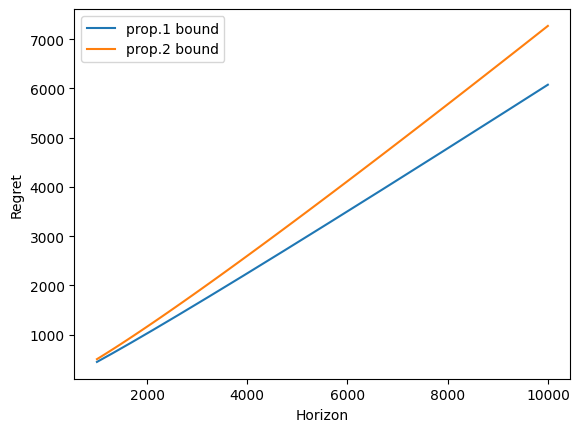
\includegraphics[width=0.8\textwidth]{graphs/proposition1-2_comparison.png}
    \caption{prop. \ref{prop:UCB_strong_lower_bound} and \ref{prop:UCB_weak_lower_bound} comparison}
    \label{fig:proposition1-2_comparison}
\end{figure}

\begin{remark}
        We get the same result of Proposition \ref{prop:UCB_strong_lower_bound} for $\pi=UCB1$ almost for free! The only change needed is in the proof of Lemma \ref{lem:arm_1_keeps_being_chosen}. The proof of Lemma \ref{lem:arm_1_keeps_being_chosen} in this case is very similar. The main thing to notice is that:
        \begin{align}
            \frac{\Delta x}{c+x}+\sqrt{\frac{2\ln{T}}{c+x}}\geq \sqrt{\frac{2\ln{T}}{c}} &\iff \frac{\Delta x}{c+x} \geq \sqrt{2lnT}\bigg(\frac{1}{\sqrt{c}}-\frac{1}{\sqrt{c+x}}\bigg)\\
            &\Longrightarrow 
            \frac{\Delta x}{c+x} \geq \sqrt{2lnt}\bigg(\frac{1}{\sqrt{c}}-\frac{1}{\sqrt{c+x}}\bigg)\\
            &\iff \frac{\Delta x}{c+x}+\sqrt{\frac{2\ln{t}}{c+x}}\geq \sqrt{\frac{2\ln{t}}{c}}
            \label{eq:iff_condition_for_keep_being_chosen_ucb1}
        \end{align}
\end{remark}

\begin{proposition}
    Let $\pi$ be the deterministic $\epsilon$-greedy algorithm such that $\frac{1}{\epsilon} \in \mathbb{N}$ and $\epsilon T \in \mathbb{N}$. Then:
    \begin{equation}
        R_\pi(\mathcal{E}, T)\geq\frac{T}{2}
    \end{equation}
\end{proposition}

\begin{proof}
    Again, we need to find an instance $\nu \in \mathcal{E}$ such that the regret is at least $\frac{T}{2}$. Fix $c \in \mathbb{N}$ such that $\epsilon c \in \mathbb{N}$ and let $\Delta \in [0, 1]$, $\alpha \in [0,1]$. The values of $c$, $\Delta$ and $\alpha$ will be determined later in the proof. Assume the two arms have the following (round dependent) distribution: $$(\mu_1(t),\mu_2(t))=\twopartdef{(\alpha,0)}{t\leq c}{(\Delta,1)}{c<t\leq T}$$
    Thus, the rewards are deterministic in each round and there is a single change point at $t=c+1$.
    Our strategy is to pick $\Delta$, $c$ and $\alpha$ such that the empirical mean of the first arm is always bigger then the empirical mean of the second arm. Our aim is to create large regret that comes from the confusion of the algorithm after the change. Lets discuss the trade offs between the parameters. Notice that $\alpha$ doesn't present any trade offs and we should always pick $\alpha = 1$. If we pick a big $\Delta$, it will take the algorithm longer to notice the change, so picking bigger $\Delta$ values will allow for smaller $c$ values hence more regret coming from after the change point. On the other hand, the regret of each round after the change would be smaller, so bigger $\Delta$ values might also cause lower regret.
    \begin{lemma}
    $$\forall t \in \{1, \ldots, T\} \quad \hat{\mu}_{t,1} \geq \hat{\mu}_{t,2} \quad \iff \quad \hat{\mu}_{T,1} \geq \hat{\mu}_{T,2}$$
    \end{lemma}
    \begin{proof}
        Of course the left side implies the right side. Assume $\hat{\mu}_{T,1} \geq \hat{\mu}_{T,2}$. Notice that $$\forall t\in \{1, \ldots, c\}, \quad \hat{\mu}_{t,1}=1\geq0=\hat{\mu}_{t,2}$$ For $t>c$, it is easy to see that the empirical mean of the first arm is decreasing while that of the second arm is increasing. Therefore for $t>c$ we have:
        $$\hat{\mu}_{t,1} \geq \hat{\mu}_{T, 1} \geq \hat{\mu}_{T, 2} \geq \hat{\mu}_{t, 2} \qed$$
    \end{proof}
    Now we find a condition for $c$ and $\Delta$ such that $\hat{\mu}_{T,1} \geq \hat{\mu}_{T,2}$.
    \begin{align}
        \hat{\mu}_{T,1} \geq \hat{\mu}_{T,2} &\iff \frac{(1-\epsilon)c+(1-\epsilon)(T-c)\Delta}{(1-\epsilon)T}\geq \frac{\epsilon(T-c)}{\epsilon T}\\ &\iff \frac{c+(T-c)\Delta}{T}\geq\frac{T-c}{T}\\
        &\iff \Delta \geq \frac{T-2c}{T-c} = 1 - \frac{c}{T-c}
    \end{align}
    Because $\Delta \in [0,1]$ we have:
    \begin{equation}
        \hat{\mu}_{T,1} \geq \hat{\mu}_{T,2} \quad\iff\quad \Delta \geq max\{0, 1 - \frac{c}{T-c}\} \label{eq:delta_condition_epsilon_greedy}
    \end{equation}
    In this case the regret is:
    \begin{equation}
        R_\pi(\nu, T) = \epsilon c + (1-\epsilon)(T-c)(1-\Delta)
    \end{equation}
    Equation \ref{eq:delta_condition_epsilon_greedy} implies that for every $c$:
    \begin{align}
        &R_\pi(\nu, T)\leq \epsilon c + (1-\epsilon)(T-c)(1-(1 - \frac{c}{T-c})) = c\\
        &R_\pi(\nu, T)\leq \epsilon c + (1-\epsilon)(T-c)(1-0) = (1-\epsilon)T+(2\epsilon-1)c\\
        \Longrightarrow & R_\pi(\nu, T)\leq max\{c, (1-\epsilon)T+(2\epsilon-1)c\}
    \end{align}
    Therefore we pick $\Delta = max\{0, 1 - \frac{c}{T-c}\}$ to maximize the regret. If $c\leq\frac{T}{2}$, then $\Delta=1-\frac{c}{T-c}$ and the regret is $R_\pi(\nu, T)=c$. Therefore in this case we pick $c=\frac{T}{2}$. If $c\geq\frac{T}{2}$, we have $\Delta=0$ and the regret is $R_\pi(\nu, T)=(1-\epsilon)T+(2\epsilon-1)c$. Because $\epsilon\leq\frac{1}{2}$, in this case, the regret is decreasing with $c$, so we pick $c=\frac{T}{2}$. Thus, in both cases we have $c=\frac{T}{2}$, $\Delta=0$, and we have $R_\pi(\nu, T) = \frac{T}{2}$. \qed
\end{proof}

%%%%%%%%%%%%%%%%%%%%%%%%%%%%%%%%%%%%%%%%%%%%%%%%%%%%%%%%%%

%%%%%%%%%%%%%%%%%%%%%%%%%%%%%%%%%%%%%%%%%%%%%%%%%%%%%%%%%%

%%%%%%%%%%%%%%%%%%%%%%%%%%%%%%%%%%%%%%%%%%%%%%%%%%%%%%%%%%

% Appendix here
% Options are (1) APPENDIX (with or without general title) or
%             (2) APPENDICES (if it has more than one unrelated sections)
% Outcomment the appropriate case if necessary
%
% \begin{APPENDIX}{<Title of the Appendix>}
% \end{APPENDIX}
%
%   or
%
% \begin{APPENDICES}
% \section{<Title of Section A>}
% \section{<Title of Section B>}
% etc
% \end{APPENDICES}

%%
%\theendnotes

% Acknowledgments here
%\ACKNOWLEDGMENT{The authors gratefully acknowledge the existence of
%the Journal of Irreproducible Results and the support of the Society
%for the Preservation of Inane Research.}


% References here (outcomment the appropriate case)

% CASE 1: BiBTeX used to constantly update the references
%   (while the paper is being written).
% \bibliographystyle{informs2014} % outcomment this and next line in Case 1
% \bibliography{mybib.bib} % if more than one, comma separated
\begin{thebibliography}{1}
    \bibitem{reference1}
        Tor Lattimore and Csaba Szepesv´ari,
        \emph{Bandits Algorithms},
        Cambridge University Press,
        2020.
\end{thebibliography}
% CASE 2: BiBTeX used to generate mypaper.bbl (to be further fine tuned)
%\input{mypaper.bbl} % outcomment this line in Case 2

%If you don't use BiBTex, you can manually itemize references as shown below.



%%%%%%%%%%%%%%%%%
\end{document}
%%%%%%%%%%%%%%%%%
